% Intended LaTeX compiler: pdflatex
\documentclass[10pt,a4paper,UTF8]{article}
\usepackage{zclorg}
\date{}
\title{本证向量与上三角矩阵}
\hypersetup{
 pdfauthor={},
 pdftitle={本证向量与上三角矩阵},
 pdfkeywords={},
 pdfsubject={},
 pdfcreator={Emacs 25.0.50.1 (Org mode 9.0.5)},
 pdflang={English}}
\begin{document}

\maketitle
\tableofcontents
\titlepic{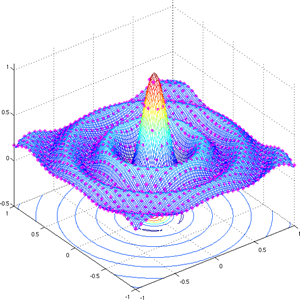
\includegraphics[scale=0.25]{../../img/sinc.PNG}}

\section{多项式作用于算子}
\label{sec:orgbe31485}


算子理论比线性映射理论更加丰富多彩,主要原因是算子能自乘为幂。我们从算子的幂以及多项式作用于算子这一关键概念的定义开始。

若\(T\in \mathcal{L}(V)\),则\(TT\)是有意义的,并且也包含于\(\mathcal{L}(V)\)。通常用\(T^{2}\)代替\(TT\),更一般的,我们有:
\begin{definition}
设\(T\in \mathcal{L}(V)\),\(m\)是正整数。
\begin{enumerate}
\item 定义\(T^{m}\)为\(T^{m} = \underbrace{T\cdots T}_{m}\)
\item 定义\(T^{0}\)为\(V\)上的恒等算子\(I\)
\item 若\(T\)是可逆的,且逆为\(T^{-1}\),则定义\(T^{-m}\)为\(T^{m} = (T^{-1})^{m}\)
\end{enumerate}
\end{definition}

\begin{definition}
设\(T\in \mathcal{L}(V)\),\(p\in \mathcal{P}(\mathbf{F})\),对\(z\in \mathbf{F}\),有\(p(z) = a_{0} + a_{1}z + a_{2}z^{2} + \ldots a_{m}z^{m}\),则\(p(T)\)是定义为\(p(T) = a_{0}I + a_{1}T + \ldots + a_{m}T^{m}\)的算子。
\end{definition}

\begin{instance}
设\(D\in \mathcal{L}(\mathcal{P}(\mathbf{R}))\)是由\(Dq = q^{'}\)定义的微分算子,\(p\)是多项式\(p(x) = 7 - 3x + 5x^{2}\),则\(p(D) = 7I - 3D + 5D^{2}\)。于是对每个\(q\in \mathcal{P}(\mathbf{R})\)有\((p(D))q = 7q - 3q^{'} + 5q^{''}\)
\end{instance}

\begin{definition}
若\(p,q\in \mathcal{P}(\mathbf{F})\),则\(pq\in \mathcal{P}(\mathbf{F})\)的定义为:\(\forall z\in \mathbf{F}, (pq)(z) = p(z)q(z)\)
\end{definition}

\section{本征值的存在性}
\label{sec:org6b80e4a}


\begin{theorem}
有限维非零复向量空间上的每个算子都有本征值
\end{theorem}
\begin{proof}
设\(V\)是\(n\)维复向量空间,\(n > 0\), 并设\(T\in \mathcal{L}(V)\),取\(v\in V\)且\(v\neq 0\),因为\(V\)是\(n\)维的,所以\(n+1\)个向量\[v,Tv,T^{2}v,\ldots ,T^{n}v\]线性相关。于是有并且为零的复数\(a_{0},\ldots ,a_{n}\)使得:
\[0 = a_{0}v  + a_{1}Tv + \ldots + a_{n}T^{n}v\]
\end{proof}
注意\(a_{1},\ldots ,a_{n}\)不全为零,否则\(a_{0}\)也必须为0.

以这些\(a_{j}\)做一个多项式,利用代数学基本定理可以将此多项式分解为:
\begin{equation}
\label{eq:1}
a_{0} + a_{1}z + \ldots + a_{n}z^{n} = c(z-\lambda_{1})\ldots (z-\lambda_{m})
\end{equation}
其中\(c\)是非零复数,每个\(\lambda_{j}\)都属于\(\mathbf{C}\),且对于式 (\ref{eq:1}) 所有的\(z\in \mathbf{C}\)均成立。则:
\begin{eqnarray}
\label{eq:3}
0&=& a_{0}v + a_{1}Tv + \ldots a_{n}T^{n}v \\
&=& (a_{0}I + a_{1}T + \ldots + a_{n}T^{n})v \\
&=&c(T-\lambda_{1}) \ldots (T-\lambda_{m})v
\end{eqnarray}

于是至少有一个\(j\)使得\(T-\lambda_{j}I\)不是单的,即有\(v\neq 0\)使得\((T-\lambda_{j}I)v = 0\),即有\[Tv = \lambda v\]

\section{上三角矩阵}
\label{sec:org46ad8e7}


\begin{definition}
设\(T\in \mathcal{L}(V)\),并设\(v_{1},\ldots ,v_{n}\)是\(V\)的基。\(T\)关于该基的矩阵定义为\(n\times n\)的矩阵:
\begin{equation}
\label{eq:4}
 \mathcal{M}(T) =
\begin{bmatrix}
A_{1,1} & \ldots & A_{1,n} \\
\vdots & \ddots & \vdots \\
A_{n,1} & \ldots & A_{n,n}
\end{bmatrix}
\end{equation}
其元素\(A_{j,k}\)定义为:
\begin{equation}
\label{eq:5}
T(v_{k}) = A_{1,k}v_{1} + \ldots A_{n,k}v_{n}
\end{equation}
\end{definition}
我们发现:
\begin{enumerate}
\item 线性算子的矩阵是正方形方阵,越来越有意思了。
\item \(Tv_{k}\)写成\(v_{1},\ldots ,v_{n}\)的线性组合时使用的那些系数构成了矩阵\(\mathcal{M}(T)\)的第\(k\)列。
\end{enumerate}

若\(T\)是\(\mathbf{F}^{n}\)的算子,且没有指定基,则假定为标准基。此时可以认为\(\mathcal{M}(T)\)的第\(j\)列维\(T\)作用到第\(j\)个标准基上得到的向量。

\begin{instance}
定义\(T\in \mathcal{L}(\mathbf{F})^{3}\)为\(T(x,y,z) = (2x+y,5y + 3z, 8z)\),则:
\begin{equation}
\label{eq:6}
\mathcal{M}(T) =
\begin{bmatrix}
2 & 1 & 0 \\
0 & 5 & 3 \\
0 & 0 & 8
\end{bmatrix}
\end{equation}
对这个问题,我们有对于标准基,显然有:
\begin{eqnarray}
\label{eq:7}
T(1,0,0)&=&(2,0,0) \\
T(0,1,0)&=&(1,5,0) \\
T(0,0,1)&=&(0,3,8)
\end{eqnarray}
\end{instance}
线性代数的一个中心目标就是要证明,对于给定的算子\(T\in \mathcal{L}(V)\),必定存在\(V\)的一个基,使得\(T\)关于该基有一个相当简单的矩阵。更直白的说法是,我们要选择\(V\)的基使得\(\mathcal{M}(T)\)有很多的\(0\),这样我们把线性映射同构于矩阵,做矩阵运算时要简单得多。


若\(V\)是有限维的复向量空间,那么可以肯定的是\(V\)有一个基使得\(T\)关于这个基的矩阵的第一列除第一个元素之外全是\(0\),也就是说,\(V\)有一个基使得\(T\)关于这个基的矩阵形状是:
\begin{equation}
\label{eq:8}
\begin{bmatrix}
\lambda & & & \\
0       & * & & \\
\vdots  &  & & \\
0       &  & &
\end{bmatrix}
\end{equation}
已知有限维复向量空间上的每个算子都有本征值,所以对于\(T\)一定有一个本征值\(\lambda\)和对应的本证向量\(v\),把\(v\)扩张成\(V\)的一个基,则\(T\)关于这个基的矩阵就具有上面的形式。

上三角矩阵的条件:
\begin{theorem}
设\(T\in \mathcal{L}(V)\),且\(v_{1},\ldots ,v_{n}\)是\(V\)的基,则一下条件等价:
\begin{enumerate}
\item \(T\)关于\(v_{1},\ldots ,v_{n}\)的矩阵是上三角的。
\item 对每个\(j=1,\ldots ,n\)都有\(Tv_{j}\in span(v_{1},\ldots ,v_{j})\)
\item 对每个\(j=1,\ldots ,n\),有\(\mathrm{span}(v_{1},\ldots ,v_{j})\)在\(T\)下不变。
\end{enumerate}
\end{theorem}

\begin{proof}
这几个命题的证明比较简单,但是证明过程需要对算子的矩阵有比较熟稔的记忆。假设\(T\in \mathcal{L}(V)\),\(T\)是\(V\)上的线性算子,则\(T\)关于该基的矩阵定义为\(n\times n\)的矩阵:
\begin{equation}
\label{eq:9}
A=
\begin{bmatrix}
A_{1,1}& \ldots & A_{1,n} \\
\vdots & \ddots & \vdots \\
A_{n,1}& \ldots & A_{n,n} \\
\end{bmatrix}
\end{equation}
其中\(A_{j,k}\)定义为:
\begin{equation}
\label{eq:10}
Tv_{k} = A_{1,k}v_{1} + \ldots + A_{n,k}v_{k}
\end{equation}
注意\(V\)上算子关于基的矩阵是一个方阵,并且\(T\)和\(V\)上的基共同决定了\(A\)。比如\(V\)上的恒等映射就是一个单位矩阵。满足:\[Tv_{k} = v_{k}\] 显然恒等映射\(T\)的特征值都是\(1\),特征向量有\(n\)个,每个都是\(V\)的基。从恒等映射我们知道一个特征值可以对应多个特征向量。好了,现在让我们回到三角矩阵的条件。

首先从第1条到第二条。因为\(T\)关于\(v_{1},\ldots ,v_{n}\)的矩阵是上三角的。所以
\begin{equation}
\label{eq:11}
Tv_{j} = A_{1,j}v_{1} + \ldots A_{j,j}v_{j} + 0 v_{j+1} + \ldots + 0 v_{n}
\end{equation}
显然\(Tv_{j}\in \mathrm{span}(v_{1},\ldots ,v_{j})\)

从第二条到第三条。
我们知道:
\begin{eqnarray}
\label{eq:12}
Tv_{1}&\in & \mathrm{span}(v_{1}) \subset \mathrm{span}(v_{1},\ldots ,v_{j}) \\
Tv_{2}&\in & \mathrm{span}(v_{1},v_{2}) \subset \mathrm{span}(v_{1},\ldots ,v_{j}) \\
&\vdots& \\
Tv_{j} &\in & \mathrm{span}(v_{1},\ldots ,v_{j})
\end{eqnarray}
假设\(v\in \mathrm{span}(v_{1},\ldots ,v_{j})\),则有 \(Tv\in \mathrm{span}(v_{1},\ldots ,v_{j})\) 也就是说\(\mathrm{span}(v_{1},\ldots ,v_{j})\)在\(T\)下不变。

第三条说明什么?说明一个上三角阵以及对应的基具有一定的嵌套性质。比如我单独的把前\(j\)列拉出来,则这\(j\)列对应的基中的元素张成了一个\(T\)下的不变子空间,自成体系。
\end{proof}

一个重要的定理:
\begin{theorem}
设\(V\)是有限维复向量空间,\(T\in \mathcal{L}(V)\),则\(T\)关于\(V\)的某个基有上三角阵。
\end{theorem}

\begin{proof}
我们使用数学归纳法。若\(\dim V = 1\),则结论是显然的,一定有\(Tv = \lambda v\)。

假设\(\dim V > 1\),并对所有维数比\(V\)小的复向量空间结论都成立。设\(\lambda\)是\(V\)的本征值,设:
\begin{equation}
\label{eq:13}
U = \mathrm{range}(T-\lambda I)
\end{equation}
我们知道\(T -\lambda I\)不是满的,因为有\(v\in \mathrm{null} (T - \lambda I)\)。根据线性映射基本定理\(\dim (T-\lambda I) + \mathrm{range}(T-\lambda I) = \dim V\) 所以\(\dim U < \dim V\).

接下来我们证明:\(U\)在\(T\)下不变。对于\(u\in U\),有:
\begin{equation}
\label{eq:14}
Tu = (T-\lambda I)u + \lambda u
\end{equation}
显然\((T-\lambda I)u \in U\), \(\lambda u \in U\) ,所以\(Tu \in U\),因此\(T\)在\(U\)下不变。

因此\(T|_{U}\)是\(U\)上的算子,有归纳法假设知,\(U\)有基\(u_{1},\ldots ,u_{m}\)使得\(T|_{U}\)对应的矩阵为上三角阵。因此对每个\(j\)都有:
\begin{equation}
\label{eq:15}
Tu_{j} = (T|_{U})(u_{j}) \in \mathrm{span}(u_{1},\ldots ,u_{j})
\end{equation}
把\(u_{1},\ldots ,u_{m}\)扩充称\(V\)的基\(u_{1},\ldots ,u_{m},v_{1},\ldots ,v_{n}\),对每个\(k\)都有:
\begin{equation}
\label{eq:16}
Tv_{k} = (T-\lambda I)v_{k} + \lambda v_{k}
\end{equation}
\(U\)的定义表明\((T- \lambda I)v_{k}\in U = \mathrm{span}(u_{1},\ldots ,u_{m})\),因此上式可得:
\begin{equation}
\label{eq:17}
Tv_{k} \in \mathrm{span}(u_{1},\ldots ,u_{m},v_{1},\ldots ,v_{k})
\end{equation}
根据式 (\ref{eq:15})(\ref{eq:17})可以知道\(T\)关于基\(u_{1},\ldots ,u_{m},v_{1},\ldots ,v_{n}\)有上三角阵。
\end{proof}
接下来给出第二种证明。
\begin{proof}
我们仍然对\(V\)的维数用归纳法。若\(\dim V = 1\),则结论显然成立。

现在假设\(\dim V = n > 1\),并设对于所有\(n-1\)的复向量空间结论成立。设\(v_{1}\)是\(T\)的任意一个本证向量,设\(U= \mathrm{span}(v_{1})\),则\(U\)是\(T\)的不变子空间且\(\dim U = 1\).

由于\(\dim V/U = n-1\),我们可以对\(T/U \in \mathcal{L}(V/U)\)用归纳法假设。于是\(V/U\)有一个基\(v_{2} + U,\ldots ,v_{n}+ U\)使得\(T/U\)关于该基有上三角矩阵。则对于每个\(j=2,\ldots ,n\),有:
\begin{equation}
\label{eq:18}
(T/U)(v_{j} + U) \in \mathrm{span}(v_{2} + U, \ldots ,v_{j} + U)
\end{equation}
对于式 (\ref{eq:18})我们有:
\begin{equation}
\label{eq:19}
Tv_{j}\in \mathrm{span}(v_{1},\ldots ,v_{j})
\end{equation}
于是,\(T\)关于\(V\)的基\(v_{1},\ldots ,v_{n}\)具有上三角矩阵。
\end{proof}

如何通过观察一个算子的矩阵来确定概算子是否可逆?如果我们很幸运的有一个基使得该算子关于这个基的矩阵是上三角的,那么这个问题就会变得很简单。

\begin{theorem}
设\(T\in \mathcal{L}(V)\)关于\(V\)的某个基有上三角矩阵。则\(T\)是可逆的当且仅当这个上三角矩阵上的元素都不是0.
\end{theorem}

\begin{proof}
设\(v_{1},\ldots ,v_{n}\)是\(V\)的基使得\(T\)关于这个基具有上三角阵:
\begin{equation}
\label{eq:20}
 \mathcal{M}(T) =

\begin{bmatrix}
\lambda_{1} & & & * \\
            &\lambda_{2} & &  \\
& &\ddots & \\
0& &       & \lambda_{n}
\end{bmatrix}
\end{equation}
我们需要证明:\(T\)是可逆的当且仅当所有\(\lambda_{i}\)均不为\(0\)
首先设对角线元素\(\lambda_{1},\ldots ,\lambda_{n}\)均不为\(0\),则有:\[Tv_{1} = \lambda_{1} v_{1}\]。因为\(\lambda_{1}\neq 0\) 所以有\[T(v_{1}/\lambda_{1}) = v_{1}\],即\(v_{1}\in \mathrm{range}(T)\)。现在对于某个\(a\in \mathbf{F}\),有:\[T(v_{2}/\lambda_{2}) = av_{1} + v_{2}\]
上式的左端和\(av_{1}\)都包含于\(\mathrm{range}(T)\),于是\(v_{2}\in \mathrm{range}(T)\)。

依次类推,\(v_{1},\ldots ,v_{n}\in \mathrm{range}(T)\),因为\(v_{1},\ldots ,v_{n}\)是\(V\)的基,所以\(\mathrm{range}(T) = V\),也就是\(T\)是满的,于是\(T\)是可逆的。

现在完成另一个方向的证明。假设\(T\)是可逆的,显然有\(\lambda_{1}\neq 0\),不然\(Tv_{1} = 0\),说明\(\mathrm{null}(T) \neq \{0\}\),这与\(T\)可逆矛盾。设\(\lambda_{j}\neq 0, 1 < j \leq n\),式 (\ref{eq:20})
表明 \(T\)将\(\mathrm{span}(v_{1},\ldots ,v_{j})\)映射如\(\mathrm{span}(v_{1},\ldots ,v_{j})\),我们知道\(\dim \mathrm{span}(v_{1},\ldots ,v_{j-1}) = j-1\), \(\dim \mathrm{span}(v_{1},\ldots ,v_{j}) = j\),所以\(T\)将一个大的空间映射到了一个小的空间,\(\mathrm{null}(T)\neq \{0\}\),所以\(T\)不是可逆的。与假设矛盾。

综上\(T\)是可逆的。
\end{proof}

值得注意的是,现在我们还无法利用算子的矩阵来精确计算算子的本征值。但是,如果我们有幸找到一个基使得算子关于这个基的矩阵是上三角的,则本征值的计算问题就变得平凡了。

\begin{theorem}
设\(T\in \mathcal{L}(V)\)关于\(V\)的某个基有上三角矩阵。则\(T\)的本征值恰为这个上三角矩阵对角线上的元素。
\end{theorem}

\begin{proof}
设\(v_{1},\ldots ,v_{n}\)是\(V\)的基,并且\(T\)关于这个基有上三角元素:
\begin{equation}
\label{eq:22}
\mathcal{M}(T) =
\begin{bmatrix}
\lambda_{1} & & & * \\
            &\lambda_{2} & &  \\
& &\ddots & \\
0& &       & \lambda_{n}
\end{bmatrix}
\end{equation}
\end{proof}

设\(\lambda \in \mathbf{F}\),则:
\begin{equation}
\label{eq:23}
\mathcal{M}(T - \lambda I) =
\begin{bmatrix}
\lambda_{1} - \lambda & & & * \\
            &\lambda_{2} - \lambda & &  \\
& &\ddots & \\
0& &       & \lambda_{n} - \lambda
\end{bmatrix}
\end{equation}
因此\(T-\lambda I\)不可逆当且仅当\(\lambda\)等于\(\lambda_{1},\ldots ,\lambda_{n}\)中的某一个。于是\(\lambda\)是\(T\)的本征值当且仅当\(\lambda\)等于\(\lambda_{1},\ldots ,\lambda_{n}\)中的某一个。
\end{document}
